\glsresetall{} 

\chapter{Discussion and Future Work}\label{chap:discussion}

\lettrine[lines=2, findent=0pt, nindent=5pt]{A}{}t the time of writing this
thesis, the \gls{pops} is still very much in development. The project began in
2021 and has undergone continuous work since then. When designing something that
is completely unique and as ambitious as a mission planning tool, it is
difficult to gauge the work required to meet its requirements. Before,
discussing future directions for the tool, it would be helpful to first go over
how \gls{pops} became what it is. 

\section{Research and the Development Process}

Early on in development, much effort was put into exploring possible tools,
languages, and frameworks to build off of. Initially, before the creation of
the Propagator service, the intention was to rely on an open-source tool,
developed by NASA, called the \gls{gmat}. \gls{gmat} is well made and designed
to model, optimize, and estimate spacecraft trajectories
\cite{hughes_using_2017}.  Originally, it was thought that it could act as a
replacement for the \gls{stk}. It could be used to take \glspl{tle} and
generate ephemerides.  \gls{gmat} comes with its own propagators and the
software could be run from the command line. Given a script representation of a
mission, ephemeris data could be generated in the form of a report.
Unfortunately, SGP4 was not supported by the software (though this was added in
a 2022 release) which made \glspl{tle} unusable given this approach.
\gls{gmat} could be expanded and has a very well set up plugin interface.
Theoretically, an open-source implementation of an SGP4 propagator could have
been implemented into \gls{gmat}.  Then the question arose, if a propagator
needed to be added, what was \gls{gmat} providing?  Upon evaluating this
approach, it was determined that using \gls{gmat} in this way added a great
deal of work. As well, some issues were: \gls{gmat} was restricted to a windows
environment, data needed to be transferred through a \gls{tcp} connection, and
generating mission scripts was convoluted. This is not to say that this time
was wasted; rather, this was time spent exploring a, what seemed to be, useful
tool that ended up being inadequate for \gls{sfl}'s purposes. 

%https://gmat.atlassian.net/wiki/spaces/GW/overview
%https://core.ac.uk/download/pdf/80605179.pdf

Similar work was done for another NASA tool called, OpenSPIFe. Its purpose was
to handle scheduling and planning. Very similar to \gls{gmat}, it provided a
great deal of functionality that could be updated and developed. Similarly,
this tool would have increased the amount of work for any developer working on
the project. For any tool that is used, developers must take responsibility for
it to at least understand how to use the tool but also make changes if bugs
appear. For both \gls{gmat} and OpenSPIFe, it was determined that the
development overhead for developing the tools from scratch would be far less
than having to maintain two tools which are fully fledged projects in their own
rights, developed by teams of professional software engineers.

Since the decision was made to move to develop a mission planning tool from
scratch, development became more productive than exploratory. The first service
developed was the Propagator service. Ephemeris data is fundamental to every
aspect of \gls{pops} so it was the top priority. Here was a situation where an
open-source library was more helpful than it was burdensome. Well tested
implementations in many languages (including Excel) of the SGP4 algorithm are
made available along with \cite{vallado_revisiting_2006}. These
implementations, though, are only of the algorithm itself and not any
surrounding functionality such as coordinate frame transforms or generating an
ephemeris. This is where a separate open-source Python implementation of SGP4
came was found. It was based on the same source code from
\cite{vallado_revisiting_2006} and it provided a library of helper functions
that enabled all of the surrounding functionality.  This allowed efforts to be
focused on validation and on using the ephemeris data rather than generating
it.

A quick note on licensing. It is of the utmost importance that a developer
conforms with the license associated with a library lest they become exposed to
litigation. Most important is whether a library requires that the source code
of the software that makes use of library must be disclosed to the public. A
`copyleft' license requires that derivative works must disclose their source
code. The \gls{gpl} license is a very common copyleft license.  Conversly, a
`permissive' license makes no obligations to derivative works. The \gls{mit}
license and Apache License are very common examples of permissive licenses.
With this in mind, much time was spent ensuring that all of the open source
tools used by \gls{pops} fell under the permissive category.  

This was especially a challenge for Cesium. Other libraries existed that
supported a 3D Earth visualization. These were very bare-bones and would
require a great deal of work to become usable. Cesium provided the most
functionality with the best \gls{api}. As such, it was worth investing time in.
Recall that CesiumJS is the open source library that most of the functionality
of the tool is built on. CesiumION is the proprietary version and provides 3D
geospatial data which includes world maps, terrain data, and specialized
objects within the viewer.  For the world map, as long as the it is
cartographically accurate, it is sufficient for \gls{sfl}'s purposes. For
example, as part of \gls{pops} there is no need for high resolution imagery of
downtown Toronto.  Similarly, there is no need for terrain data for a space
application.  Time was spent looking for free alternatives, which were found.
As such, there was no reason to pay for a license to CesiumION when free
alternatives existed.

After Cesium was made usable, most of the tools were in place to begin full
development of \gls{pops}. This began with foundational work setting up a basic
website that could be interacted with. Initially, it was very simple and had a
number of menus that could be used to create missions, add satellites, add
ground stations, and configure a plan. From this began work on the observation
configuration page which was the most complicated aspect of \gls{pops} yet
developed. It needed to interact with all the tools that had been introduced.
Not only that but it also needed to search for opportunities.

Opportunity searching was the most difficult aspect of \gls{pops}. It is
completely unique, in that there existed no open-source tool that could be
configured to find remote sensing opportunities given some constraints. Of
course, \gls{stk} could be used, but it would require a license and would need
to be automated in some way. Other tools like \gls{cpaw} could be used but
again they provided superfluous functionality and required licenses. This
process would need to be done from scratch. Before beginning development, a
document was written that fully defined all of the initial observation modes
that were desired as part of \gls{pops}. Information like: what satellites were
necessary for a particular observation; can one, some, or all be used;
explicitly defining what constraints were necessary; defining what terminology
was being used; etc. This document was then reviewed to ensure that there was a
correct understanding of what was required.

Originally, just the \gls{atu} were thought to be sufficient for opportunity
filtering. Through, the creation of this reference document, it became clear
that in isolation, the \glspl{atu} could not fully constrain the observation
modes as described in the document. Strung together, they could do so.  This is
how the flow-charts similar to Figures~\ref{fig:filter-1} and
\ref{fig:filter-2} from Chapter~\ref{chap:intro} were created. They summarized,
at high level, how the \glspl{atu} could be used to fully constrain an
observation. They were easy to understand and make changes to. It followed that
the implementation of the opportunity filter should be as simple as these high
level diagrams. In response, the filter was split into a number of classes that
emulated the flow-diagrams. The Data Handler classes represented the data at
varying stages, such as the: Ephemeris, \gls{aoi}, Swaths, Polygons, and Access
Times. The \gls{atu} Handler, could use the data handler classes as inputs and
outputs. Finally the Opportunity Filter class would use the other two classes
to fully implement a filter.  

Implementing these filters required iteration. Not just for efficiency but also
because each version made assumptions about the filters that artificially
limited the filter's capabilities.  It is very difficult to plan and account
for each aspect of the filters before hand.  For example, the temporal
properties of the Tip-and-Cue Imaging observation had some hidden challenges.
From a high level, it is very simple: (1) first pass tip access, (2) ground
contact, and (3) next pass cue access. The initial solution may be to iterate
through each pass for a scenario. For each pass, we find the access time
between Sat-A and the \gls{aoi}. Then we calculate an access between Sat-B and
the intersection polygon from the Sat-A \gls{aoi} access. Then if that access
exists and if there is a ground contact, all the information is stored as an
opportunity. This is essentially what is currently being done as outlined in
Algorithm~\ref{alg:tip-and-cue} in Chapter~\ref{chap:architecture}.  

This solution is technically valid, but what if there are multiple Sat-A
\gls{aoi} accesses in a single pass? Or, what if there are multiple Sat-B
intersection polygon accesses? Then, this process of iterating over passes may
miss potential opportunities. Now, we need to improve the solution and instead
of looping over every pass, we iterate over every Sat-A \gls{aoi} access.  In
this way, we never miss a tip opportunity. Then, we intersect the tip
intersection polygon with the first Sat-B intersection polygon on the next
pass.  This is just one example of how the process needs to be iterated.  Other
sources were effectively managing the data in a scenario.  Specifically how
should data be stored such that it can be used as needed throughout the
filtering process, how to prevent copying the data unnecessarily, or also how
to provide data to the \glspl{atu} effectively such that the filter wasn't
slowed down unnecessarily by performing repeated or superfluous calculations.  

%The last area that slows down development is bug fixing and stability
%improvements. This nothing special; any part of a development workflow will
%require ironing out bugs. Given the scale of the tool, part of the attitude
%when developing has been making things perfect takes a lot of time so make it
%good enough to work for now. This is perfectly valid, and makes sense.  There
%is neither the time nor the resources to support optimizing every aspect of
%the tool. That being said, expanding the tool requires building on itself.
%Much of the functionality is inter-reliant and very little can be done in
%isolation. If we fully followed a ``get it done'' mentality, the tool would
%quickly fall in on itself. For this reason, a great deal of time has been
%spent iterating on every aspect of the tool to make it more robust, such that
%when new functionality is added, it is not limited artificially or it does not
%cause the tool to collapse in on itself.



\section{Future Work}

Now, with some understanding for how \gls{pops} was created, we now can go over
some areas where \gls{pops} needs to be developed and improved. Some of these
are critical updates that are necessary for the \gls{mvp} and others are
important for the general health and functionality of the tool.

\subsection{Time Tag Command Generation}

The number 1 most critical aspect of \gls{pops} that must be developed is the
\gls{ttc} generation functionality of \gls{pops}. It is an essential component
of the tool and cannot be omitted. There are two aspects to this, first, the
functionality must be developed and, second, the necessary \glspl{ttc} for each
observation mode must be determined.

Work has been done to implement \gls{ttc} generation. There exists a library
developed by \gls{sfl}, written in Python, that handles the logic for creating
\gls{nsp} commands. Work was done to re-tool this library to generate
\glspl{ttc} from these \gls{nsp} commands. A service was created around the
re-tooled library to generate list of \glspl{ttc} for each observation mode.
The intention for this service was to be expandable and easy to use for future
developers since what \glspl{ttc} are used for each observation mode will
change from mission to mission. This where the intricacies discussed in
Section~\ref{sec:ttc-gen} where discovered. Unfortunately, it was decided that
using Python scripting to generate \glspl{ttc} may be too complicated or
cumbersome for future developers. In addition, the \gls{nsp} library did not
explicitly track the data payloads of the \gls{nsp} commands. That is, the
library could construct valid commands but they did not track mission-specific
information. Typically, for ground software at \gls{sfl} this is handled by
\gls{xml} configuration files that need to be configured for each new mission.
The \gls{nsp} library did not make use of these configuration files because it
was made for testing and not necessarily for nominal operations. So, when using
the Python \gls{nsp} library, individual data bits would need to be specified
in Hexadecimal. Despite the amount of work put into this new service, it was
decided that these issues were irreconcilable with the future needs of
\gls{pops}. So the service was replaced by a new tool that builds off of
\gls{xml} configuration files as the foundation for \gls{ttc} generation. This
tool is still in development.

Determining what commands are necessary for each observation mode is difficult.
Necessary commands may be: powering on devices in the spacecraft, setting
profiles, arming and disarming these profiles, specifying where in memory where
data should be stored, specifying the necessary duration for commands,
specifying attitude modes, etc.  There does not exist a single reference for
what commands are necessary and what must be done for an observation mode. This
information can only be gained through discussion with operators and with
software engineers developing the firmware.  Even after extensive consultation,
steps may be missed. It is only through testing, do we determine all of the
necessary commands for an observation mode.  Thankfully, much of this testing
can be done during \gls{tvac} testing campaigns. It is here, were spacecraft
may be commanded to perform observations, or at least their ground analogues,
through \glspl{ttc}. This gives a great deal of information about what exactly
needs to be performed for each observation. It also provides some means of
validating \gls{ttc} generation.


\subsection{Validation}

The next most important aspect of \gls{pops} that must be accomplished before
an \gls{mvp} is ready, is validation. We must ensure that the tool yields
acceptable and accurate results. System level validation can be accomplished
through service-level verification. This has been touched on throughout the
thesis. Specifically, the Propagator service was validated through comparing
ephemeris data with results from \gls{stk}. \gls{ttc} generation validation may
be accomplished through \gls{tvac} testing. After this validation becomes
difficult. The \glspl{atu} may must be individually validated either through
known test cases or through comparissons with \gls{stk}. This process has been
handled separately. Opportunity filtering is especially difficult to validate
since there does readily exist an alternative that can act a benchmark. In the
future, what may be done is when the filtering process heas reached maturity,
simple test scenarios will be constructed for each observation mode. \gls{stk}
and \gls{pops} will separately be used to search for opportunities and these
results will be compared. Thankfully, there is not a requirement for some of
the components. For example, a high accuracy with respect to access times is
not necessary. Even if the access time calculation were made very accurate,
there are inherent uncertainties in the ephemeris data that may render such
accuracy useless. This all being said, validation strategies is an ongoing
process.
 
%\subsection{Addition of More Observation Modes}
%
%Some missions that \gls{pops} is intended to be used for require additional
%operations modes beyond just what was discussed in the 

\subsection{Performance}

Currently \gls{pops} has issues with large amounts of data. For scenarios
longer than a few days, storing and retrieving data, displaying information,
and opportunity filtering becomes slow. To illustrate this, let us run a simple
benchmark test. For this test, we will run the Tip-and-Cue Imaging opportunity
filter for a number of scenarios, each with an increasing scenario size and a
10s timestep. Each scenario will have two satellites (Sat-A and Sat-B), three
ground stations (\acrshort{sfl}, ESCS, and GSW), and the same \gls{aoi}
discussed in Chapter~\ref{chap:workflow}. The reason we'll use the opportunity
filter as a benchmark is that it interacts with almost every part of \gls{pops}
and Tip-and-Cue Imaging is the more complicated observation mode.
The purpose of this test is not to give an in-depth characterization of the
performance of \gls{pops} but rather its purpose is to give a rough idea.
These scenarios were run on a laptop with 40GB of RAM and an $11^{th}$
generation Intel Core i7-1165G7 CPU running at 2.80 GHz. 


\begin{figure}[h]
    \centering
    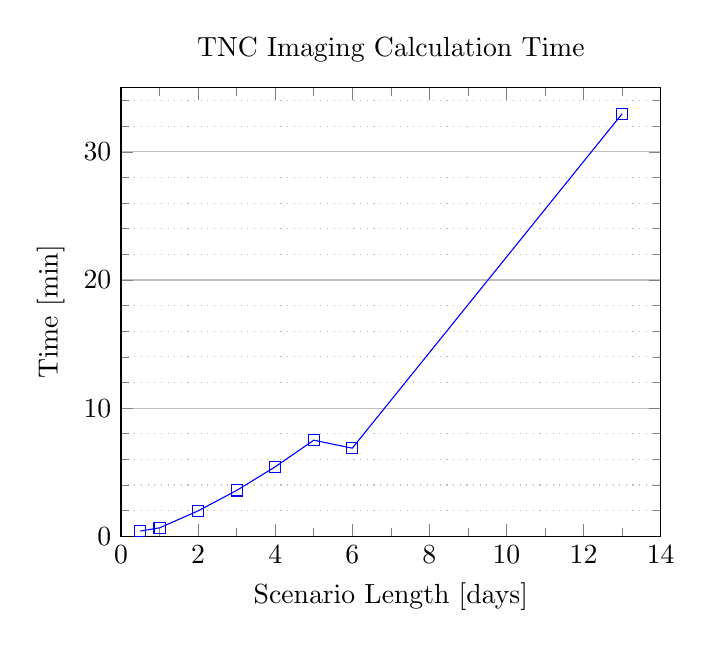
\begin{tikzpicture}
    \begin{axis}[
	title={TNC Imaging Calculation Time},
	xlabel={Scenario Length [days]},
	ylabel={Time [min]},
	xmin=0, xmax=14,
	ymin=0, ymax=35,
	xtick={0, 2, 4, 6, 8, 10, 12, 14},
	minor x tick num=1,
	minor y tick num=4,
	ymajorgrids=true,
	yminorgrids=true,
	minor grid style=dotted,
    ]

    \addplot[
	color=blue,
	mark=square,
	]
	coordinates {
	(0.5, 0.400643333) (1, 0.651415) (2, 1.976971667) (3, 3.57072) (4, 5.415478333) (5, 7.492456667) (6, 6.871896667) (13, 32.980525)
	};
	
    \end{axis}
    \end{tikzpicture}
    \caption{Simple Opportunity Filtering performance benchmark}
    \label{fig:performance-benchmark}
\end{figure}

The results of this test can be seen in Figure~\ref{fig:performance-benchmark}.
As can be seen from the plot, 8 scenarios were generated. Scenarios less than 4
days are reasonably quick, taking less than \~5 minutes. But, as we approach a
13-14 day scenario filtering takes more than half an hour. It could be argued
that this is tolerable for an \gls{mvp} but it is certainly not ideal.  Note,
this test was only for a 2-satellite scenario. Every satellite added increases
the running time exponentially. 

To address this, there are a number of areas for improvement.  These range from
simple algorithmic changes to heavily involved architectural changes. For each
change, work will need to be done characterizing what is taking up the most
time to justify the change. Some possible avenues for improvement, in increasing
difficulty, are:

\begin{enumerate}
    \item Making ephemeris data dynamic,
    \item Splitting up the data in the filtering process,
    \item Utilizing parallel computation,
    \item Offloading computation to a dedicated server, or
    \item Leveraging the GPU
\end{enumerate}


\subsubsection{1. Making Ephemeris data dynamic}

As mentioned earlier, ephemerides are generated for each satellite once when a
plan is created. This ephemeris data has a set time range and timestep. It is
here a user must decide whether they want an accurate but slow to process plan,
or an inaccurate but fast plan. Why should they be required to make this
decision? Or, at least, why should this decision be made once and then be set
in stone for the duration of the plan? What's more, if the timestep is constant
for an entire plan, it is likely that, for small timesteps, most of that data
is wasted. If a user is concerned with an \gls{aoi} in the Northern Hemisphere,
they will not need a high accuracy ephemeris for times where the spacecraft is
in the southern hemisphere. Of course, if the user is concerned with a very
large \gls{aoi} that the spacecraft more often than not has access to, then
nothing can be done but this is an outlier case.

This touches on potential improvements for how ephemerides can be better
handled.  Instead of initially making a large, small timestep, ephemeris, a
rougher, large timestep, ephemeris could be generated. For periods where high
accuracy is needed, such as when there is an access, ephemeris data could be
dynamically generated in that area specifically to increase the accuracy where
it is needed. Or, conversely, a small timestep ephemeris could be initially
generated, then after the calculations are performed, unnecessary data could be
omitted. These are both general ideas for now and would need dedicated
development time to plan out and troubleshoot any pitfalls.

In terms of difficulty, this would require a re-work of a large portion of
\gls{pops}.  Thankfully, through abstracting how ephemeris data is handled
through the Data handler class, \gls{pops} is well situated for this change.
Overall, this is a change that should likely be made anyway. Having ephemeris
data be static artificially limits \gls{pops}'s functionality.


\subsubsection{2. Splitting up data in the filtering process}

Currently, during opportunity filtering, all of the data is loaded for the
entire scenario. That being ephemeris data, swaths, access times, etc. If
having all of this data loaded in at once is causing the filtering process to
slow down, it may be better to instead load the data in chunks. For example,
for a 14 day scenario, instead of loading in all 14 days of data, this could be
split up into 2 day chunks. This will likely not reduce the processing time but
it may reduce the time spent indexing and accessing the data. In terms of
difficulty, this would be an easy modification but time would need to be spent
determining whether this actually addresses a problem in the software.


\subsubsection{3. Utilizing parallel computation}

Moving from single-threaded processing to multi-threaded processing begins to
stray from algorithmic changes to changes in how the host PC's is utilized.
These solutions, while most likely effective, increase the complexity of
\gls{pops} and should be pursued if there are no other alternatives.

Thankfully, opportunity filtering is well suited for multi-threaded
programming. Searching for opportunities is done through brute-force numerical
computation, and many of the calculations are performed independently from each
other. A system could be developed that splits the filtering process into a
number of processes, each handling sub-components of the filtering process. 

This would be a difficult solution to implement. Multi-threaded programming is
not necessarily complicated in Python, but asynchronous processes are almost
always much more complicated that asynchronous process. Synchronous processes
are predictable, straightforward, and easy to debug. Asynchronous processes
introduce a multitude of challenges. For example: race conditions, memory
management, locking out resources, unpredictable behavior, error handling, etc.
There are many benefits to parallel computing, but such a change should not be
undertaken lightly.


\subsubsection{4. Offloading computation to a dedicated server}

When performing opportunity filtering, or any other function of \gls{pops}, if
other software is being run on a user's computer, that may negatively impact
the tool's performance. Or, if the user's computer is not particularly
powerful, that may limit \gls{pops}'s usefulness. Instead, a dedicated server
could be constructed that is optimized to perform calculations for \gls{pops},
such as ephemeris generation, the \glspl{atu}, database management, and
opportunity filtering. In this way, all that a user's computer will run is what
they need to display the information or construct requests. Or alternatively,
all of \gls{pops} could be hosted on a server, and a user just sends requests
to it. 

There are potential benefits to this approach, but it would vastly increase the
complexity of \gls{pops}, especially for the front-end user interface. Some
difficulties would include: managing data transfer, tracking user sessions, or
potentially removing functionality from the Mission Model service. The issue of
tracking user sessions is particularly difficult. If a user runs \gls{pops} on
their own computer, it can be assumed that only they will be interacting with
the webserver. But, if the server is hosted remotely, then the webserver needs
to track both what requests are being sent to it as well as from what source.
For example, let us say there are two users who wish to work with two different
plans. User 1 will open Plan A and the webserver will display Plan A. User 2
will open Plan B and Plan B will be displayed. But now there are two instances
of the Cesium viewer. Which one should the server send data to? The behavior is
undefined and both User 1 and User 2 will have unstable sessions. In this way,
sessions should be split somehow, such that one user's inputs cannot affect
another user. This problem has many solutions but is non-trivial and strays
into professional web development which is not the priority for \gls{pops}. 


\subsubsection{5. Leveraging the GPU}

So far, all computation has been done on the \gls{cpu} which is general purpose
but slow. The \gls{gpu} is optimized for computer graphics and image
processing. Specifically, they are built to process large blocks of data in
parallel. They are especially good at handling any process that uses linear
algebra. Historically, \glspl{gpu} were only meant to be used for computer
graphics but in recent decades, they have become much more general purpose. By
leveraging the \gls{gpu}, computation times may be decreased by orders of
magnitude. Some precedent does exist for this by accelerating SGP4 calculation
\hl{cite}.

% https://core.ac.uk/download/pdf/301091034.pdf
% https://amostech.com/TechnicalPapers/2016/SSA-Algorithms/Moeckel.pdf

Using a \gls{gpu} would be the most rewarding but also most difficult and
complicated improvement to \gls{pops} that could be made. Writing code for a
\gls{gpu} is to some extent specific to the manufacturer and age of the
\gls{gpu}. Some computers that may run \gls{pops} may not even have one that
supports this functionality. So in addition to creating the custom shaders for
\gls{pops}, work would need to be done to ensure that they can be used at all
by users at \gls{sfl}.
 

\subsubsection{Miscellaneous Improvements}

In addition to any large improvements, there exists many smaller changes that
can have a positive effect on \gls{pops}'s performance. Small changes such as:
dynamically loading data from the database, sending multiple batches of data to
the \glspl{atu} in a single HTTP request rather than multiple HTTP requests,
or.


\subsection{Updating Plans}

Another area that must be improved is the ability to update plans in
\gls{pops}. Currently, once \glspl{tle} are set for a plan, they cannot be
changed. This was done to reduce the complexity of the tool. This is not ideal
though. Suppose a plan has been made and observations have been scheduled, but
then suppose after some time a new \gls{tle} is generated that invalidates the
observations made with the older \gls{tle}. This is a reasonable scenario that
could very well occur but currently there is no way to handle this in
\gls{pops} aside from creating a new plan and rescheduling observations.

This is a multi-faceted problem that must be addressed in a number of areas.
First, we must at least determine if a new \gls{tle} invalidates observations
from a plan with a previous \gls{tle}. Next, there must be a way to edit
observations in an old plan, or there must be a way to migrate those old
observations to a new plan with updated timings. Lastly, if a change is made to
an observation, \glspl{ttc} that have already been generated must be updated in
some way to reflect the changes. This problem has not yet been approached and
is an on-going limitation of the tool.


\subsection{Communication With Other Ground Software}

\gls{pops} is not meant to be used in isolation. It is important that it is
able to communicate with other ground software at \gls{sfl}. Specifically,
\gls{pops} must be able to read what commands are currently scheduled for
different spacecraft. This is necessary for planning and for scheduling.
Without an understanding of what is already planned for a satellite,
observations that a user adds may conflict with existing \glspl{ttc}. 
How exactly \gls{pops} will interact with \gls{sfl}'s ground software has yet
to be determined.  

This additional functionality is planned to be an additional class which acts
as an interface between the scheduler class and \gls{sfl}'s ground software. It
is here uploaded \glspl{ttc} will be read and added onto the schedule.



\subsection{Testing}

The last task that must be performed before \gls{pops} has reached the
\gls{mvp} is user testing. Quite simply, this is where operators begin to use
the tool and give feedback. This information is critical since it gives
information: bugs, user interface problems, and what parts of the tool can be
improved.  This then begins the process of iterating in their feedback,
improving the tool, receiving further feedback and so on.


